%\chapter{det-comp}


%%%%%%%%%%%%%%%%%%%%%%%%%%%%%%%%%%%%%%%%%%%%%%
%\section{Anode Plane Assemblies}

%%%%%%%%%%%%%%%%%%%%%%%%%%%%%%%%%%%%%%%%%%%%%%
%\section{Cathode Plane Assemblies}

%%%%%%%%%%%%%%%%%%%%%%%%%%%%%%%%%%%%%%%%%%%%%%
%\section{Field Cage}

%%%%%%%%%%%%%%%%%%%%%%%%%%%%%%%%%%%%%%%%%%%%%%
\section{HV components}

The TPC high voltage components include the HV power supply, cables,
filter circuit, feedthrough, attachment to the resistive cathode plane
arrays, the HV bus providing low-resistance connections between CPAs,
connections to the field cage, and devices for monitoring steady state
and transient conditions of current and voltage.

A schematic of the complete TPC HV circuit is shown in Fig.\ \ref{fig:TPCHVcircuit}.

\begin{cdrfigure}[TPC HV circuit]{TPCHVcircuit}{A schematic of the TPC high voltage circuit.}
  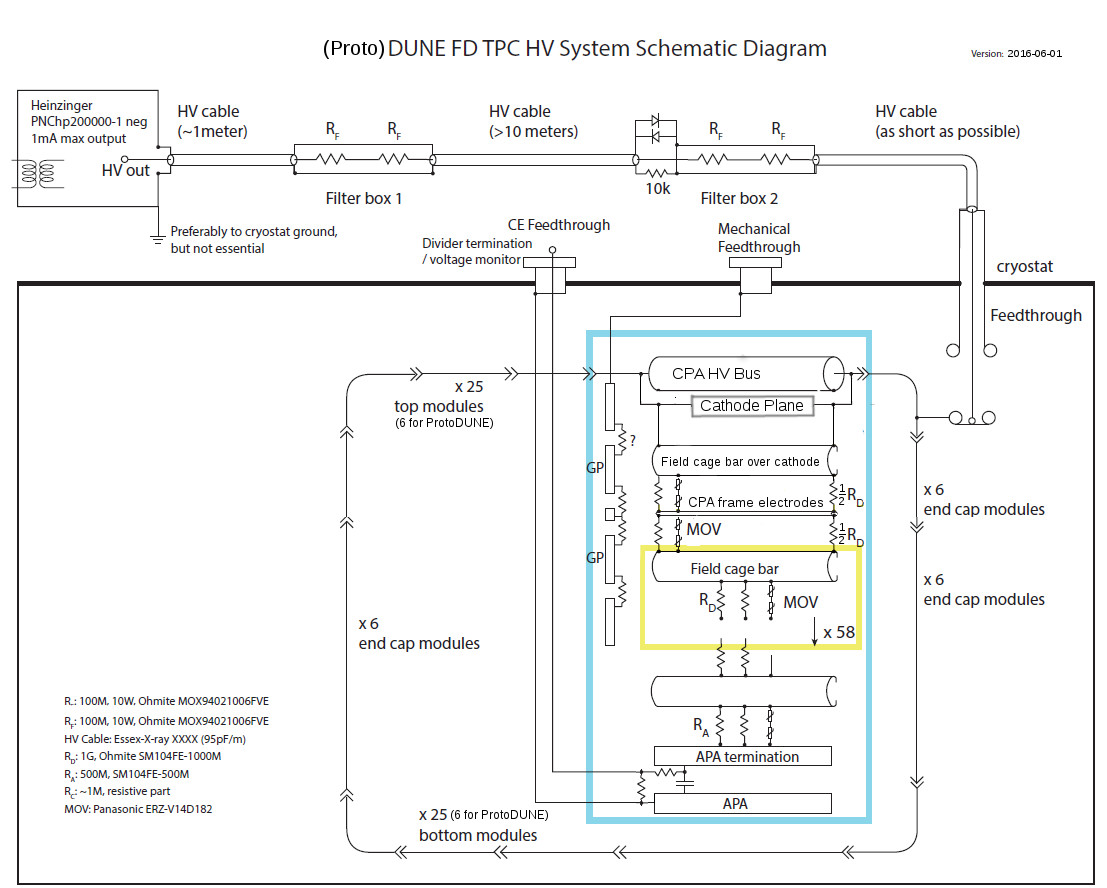
\includegraphics[width=0.75\textwidth]{VR_TPC_HV_schem-mod-1}
\end{cdrfigure}


The cathode plane will be biased at \SI{-180}{kV} to provide the
required \SI{500}{V/cm} drift field.  It will be
powered by a dedicated HV power supply through an RC filter and
feedthrough.  The power supply for the cathode plane must be able
to provide \SI{-200}{kV}.  The output voltage
ripple must not introduce more than 10\%\fixme{(?) check ripple requirement}
of the equivalent thermal
noise from the front-end electronics. The power supply must be
programmable to shut down its output at a certain current
limit. During power on and off, including output loss (for any
reason), the voltage ramp rate at the feedthrough must be controllable
to prevent damage to the in-vessel electronics from excess charge
injection. The high-voltage feedthrough must be able to withstand \SI{-250}{kV}
at their center conductors in a \SI{1}{atm} argon gas environment when
terminated in liquid argon.

%% input from F. Pietropaolo

\subsection{HV feedthrough design, Power supply, cabling}
In the present baseline option, the design of the HV feedthrough, the procurement of the Power supply and HV cables and possibly the HV filtering scheme, will take advantage of the strong synergies between Single phase and Double phase prototypes.

\begin{itemize}	
\item The Heinzinger 300 kV power supply (residual ripple less than $10^{-5}$) and the related HV cable foreseen for the DP detector are also well suited for the SP although used at lower voltage.
\item The present DP HV feedthrough design is easily adapted to the SP without any major modification in the dimensions or in the mechanical features.
\item The filtering scheme and the monitoring system is probably more demanding on the SP detector, due to the more sensitive front-end electronics, however a common development with the DP could be advantageous, allowing to get the same HV distribution chain for both the SP and the DP protoDUNE detectors.
\item Common spare components are also envisaged.
\end{itemize}

The present design of the 300 kV feedthrough is based on the very successful construction technique adopted for the ICARUS HV feedthrough, which was operated at 75 kV uninterruptedly of more that three years without any failure. The feed through was also successfully operated for several days at 150 kV.  
A coaxial geometry is adopted: the design is based on an inner conductor (HV) and an outer conductor (ground) insulated by UHMW PE  as shown in Figure~\ref{fig:hv-feed-through}. The outer conductor, made of a stainless-steel tube, surrounds the insulator extending inside the cryostat up to the LAr level. By such a geometry the electric field is always confined in regions occupied by high dielectric strength media (UHMW PE and LAr). The inner conductor is made of a thin wall stainless-steel tube, in order to minimize the heat input and to avoid the creation of argon gas bubbles around the HV lower end. A contact, welded at the upper end for the
connection to the HV cable and a round-shaped elastic contact for the connection to the cathode, screwed at the lower end, completes the inner electrode. Special care has been taken in the assembling to ensure the complete filling with the PE dielectric of the space between the inner and the outer conductors and to guarantee leak tightness at ultra-high-vacuum level.

The design of the full HV chain foreseen for the DP detector, will be finalised  after a series of tests on a prototype feed through and on the Heinzinger 300 kV Power Supply, which are presently ongoing at ETHZ and CERN. An alternative but similar design for the HV feedthrough is also under development at UCLA. Final decision on the design options will be based on max reachable HV, reliability /stability at design HV, residual noise performance.


\begin{cdrfigure}[HV feed-through]{hv-feed-through}{Preliminary design of the DP HV feed-through.}
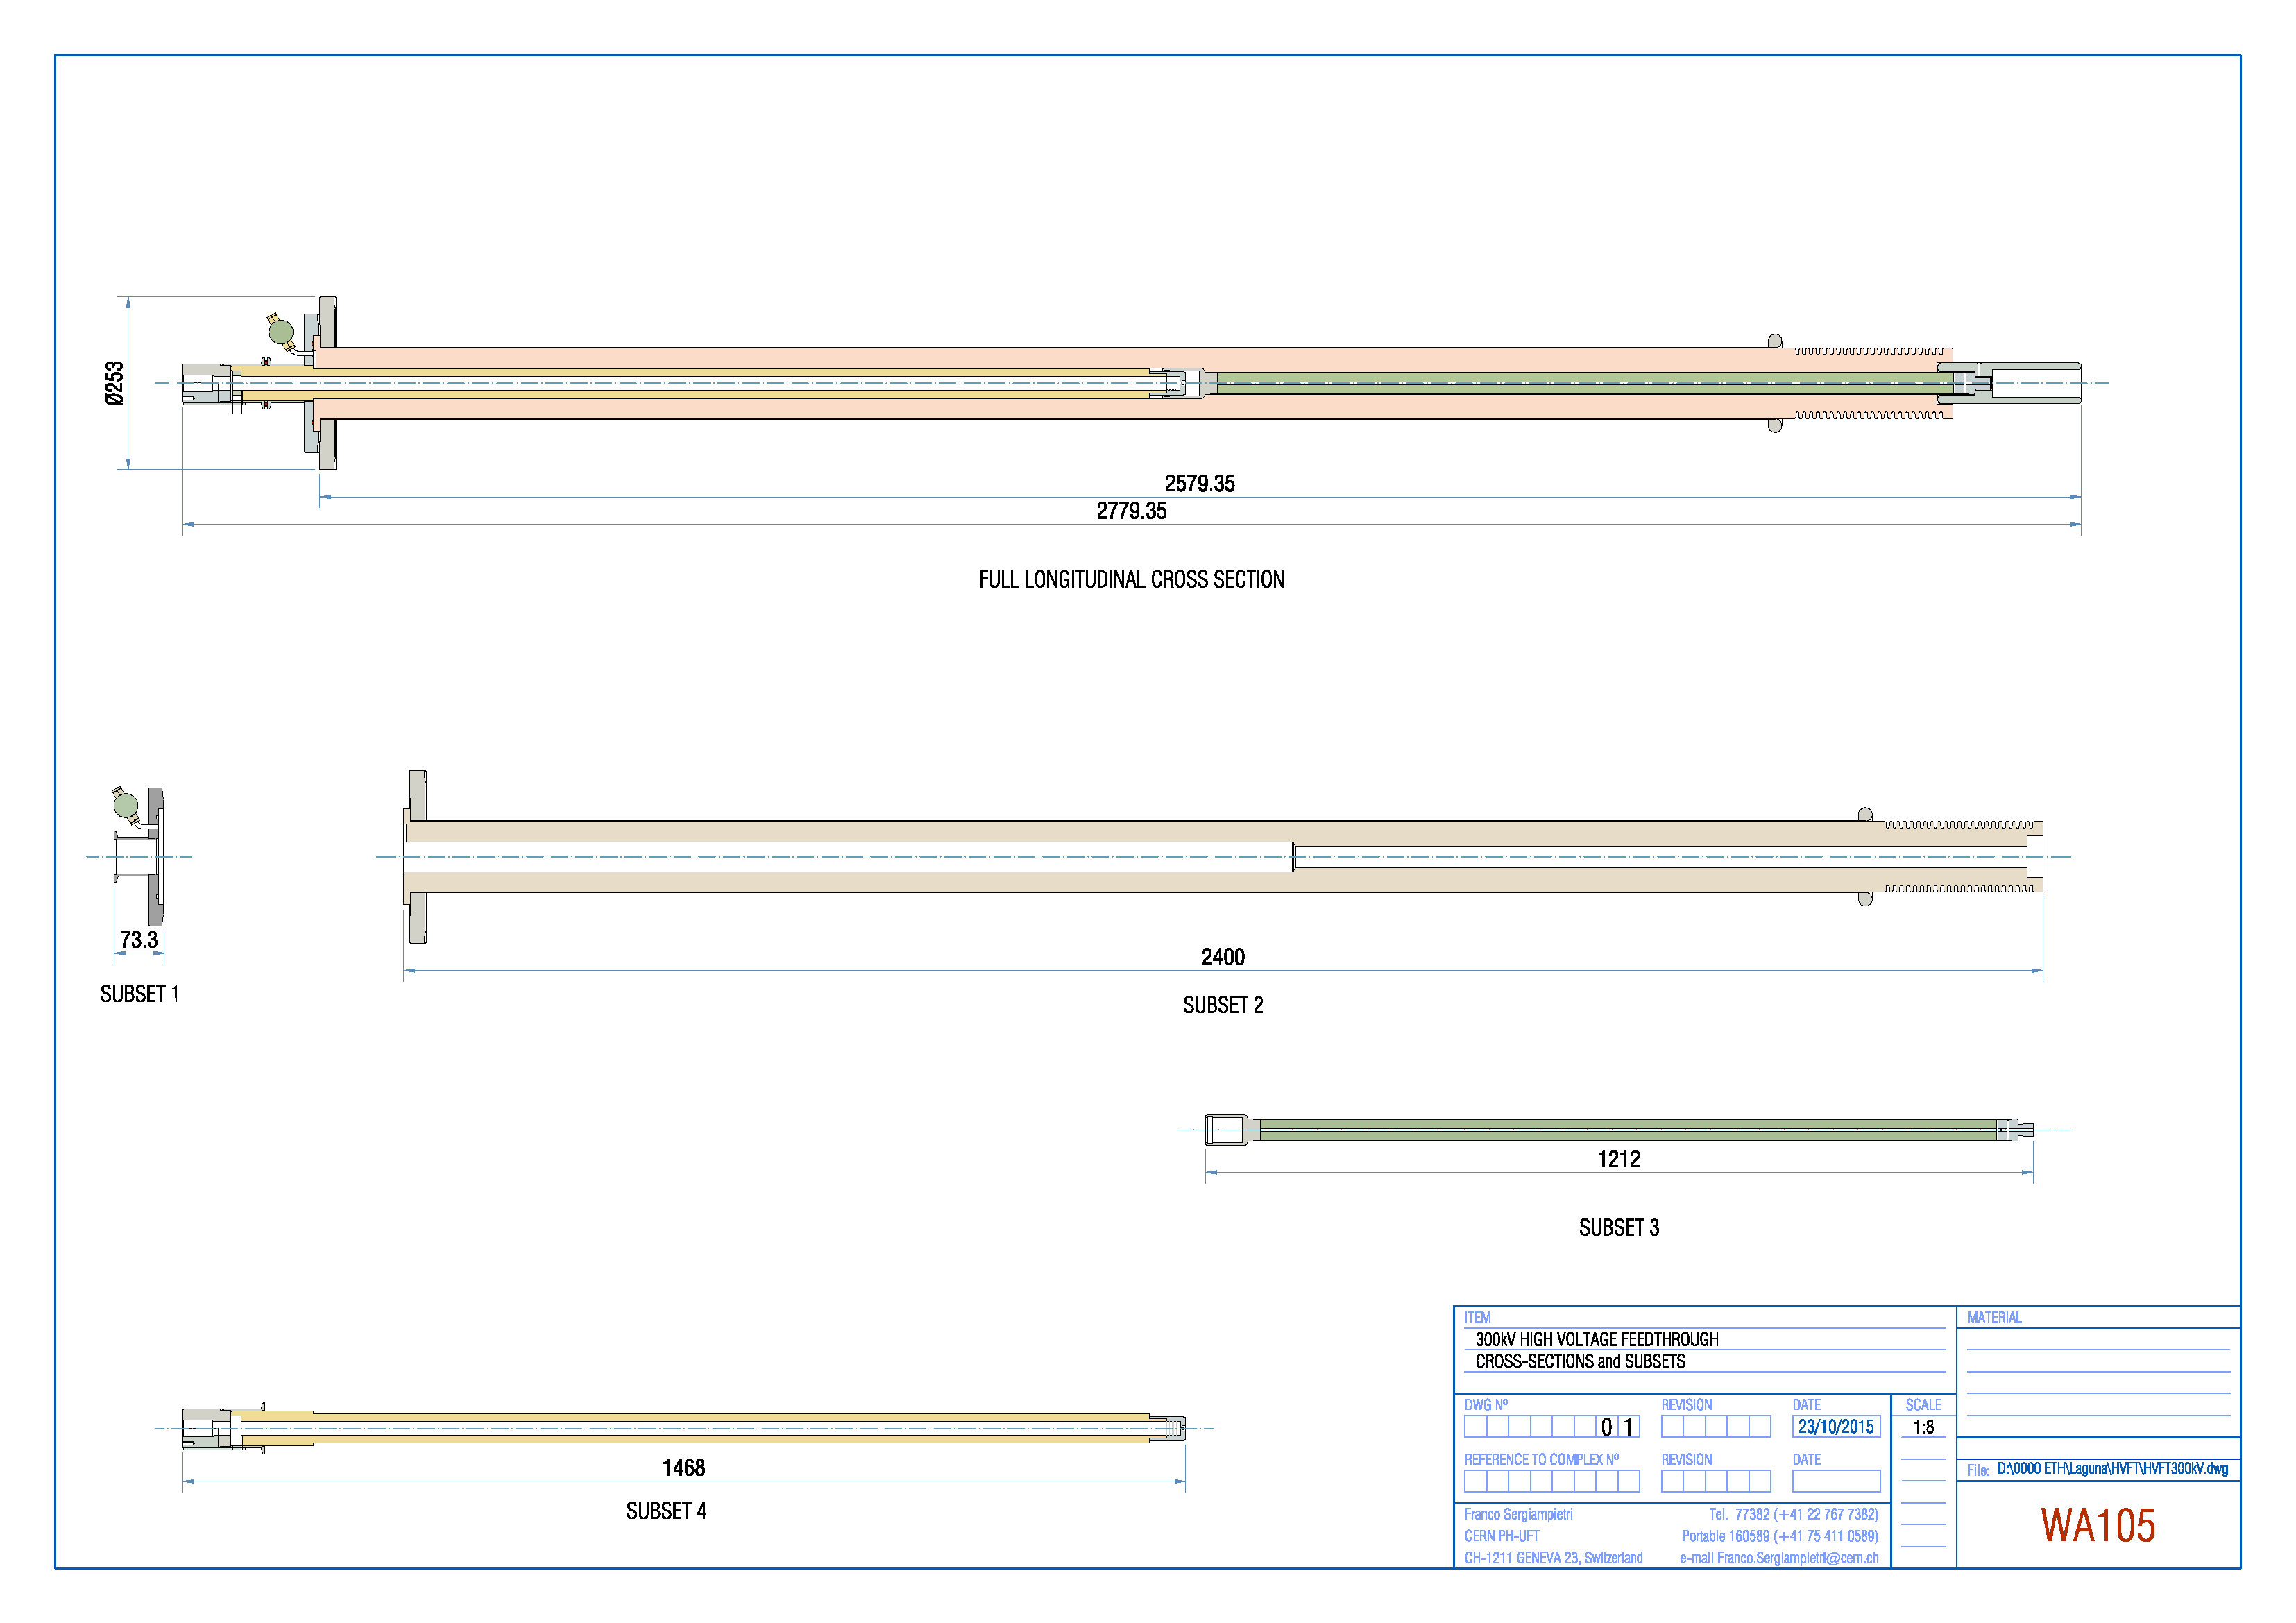
\includegraphics[width=0.8\linewidth]{tpc_HVFT300kV-1.png}
\end{cdrfigure}

%%


Despite of the ripple spec of $10^{-5}$ from the Heinzinger power supply, the ripple amplitude is still too large for the TPC.  At 2.5m drift distance (the short drift configuration), the capacitive coupling between the cathode and the grid plane, assuming a simple parallel plate capacitor, is about 73~pF.  About 20\% of this coupling goes to the first induction plane (U).  There are 800 U wires per APA, each wire faces the CPA with half of its length. So the capacitance between a U wire and the CPA is about 18~fF.  To inject 100e noise into a U channel, it only needs about 0.9~mV of ripple on the cathode.  While the power supply at 180~kV will generate ripple voltage of 1.8~V.  Obviously for the SP TPC, further filtering of the HV output with attenuation factor of $>2000$ is needed. 

%The current candidate for the high-voltage power supplies is the 
%Heinzinger PNChp series, which has the lowest output ripple 
%specification.
Additional filtering of the voltage ripples is done
through the intrinsic HV cable capacitance and series resistors
installed inside the filter box. Established techniques and practices
will be implemented to eliminate micro-discharges and minimize
unwanted energy transfer in case of an HV breakdown.

%We have two current candidates for the feedthrough: a feedthrough
%designed by and under construction at UCLA, and the dual-phase
%feedthrough design.

\subsection{HV Bus}

As described in the CPA section above, the cathode planes will be
resistive, with electrical connections at the corners, in order to
control the energy delivered in any discharges.  A low resistance
``high voltage bus'' will provide the high voltage to the field cage
circuit and cathodes with voltage drop much less than 0.1\% of the
cathode voltage.  Field-shaping electrodes on the faces of the CPA
frames will be part of the field cage circuit, described in the field
cage section above. Field cage electrodes on the outer edges of the
CPA frames will be held at the cathode potential to provide field
uniformity and to protect the HV bus from discharge.  The feedthrough
will connect to a high voltage cup on one side of a CPA at one end of
the cathode plane.  Interconnection of the bus between CPAs will be
through HV cables passed through the CPA frames.  See
Fig.~\ref{fig:HVbus} for drawings of the high voltage bus and its
interfaces.

\begin{cdrfigure}[Drawings of the HV bus.]{HVbus}{Top: A perspective view of CPA frame showing the location of the HV bus cable and attachments to the HV cup and resistive cathode, with CPA frame electrodes omitted to make HV bus visible. Middle: A sketch showing interconnection between two CPAs. Bottom: A transverse cross-section with equipotential lines around the HV bus and CPA frame.}
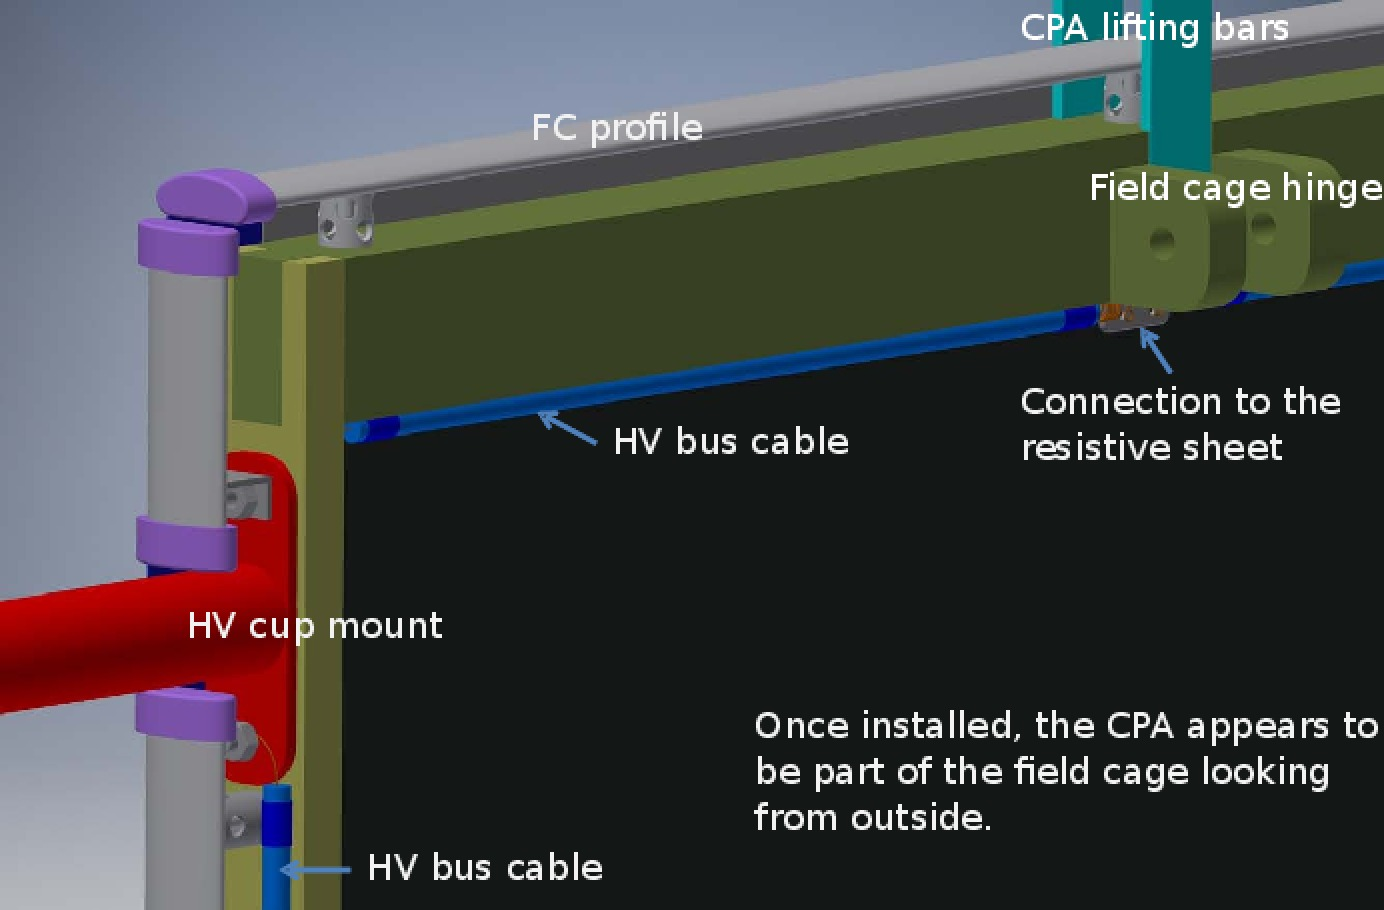
\includegraphics[height=0.29\textheight]{DUNE_SP_CPA_Design_Update-slide17-mod}
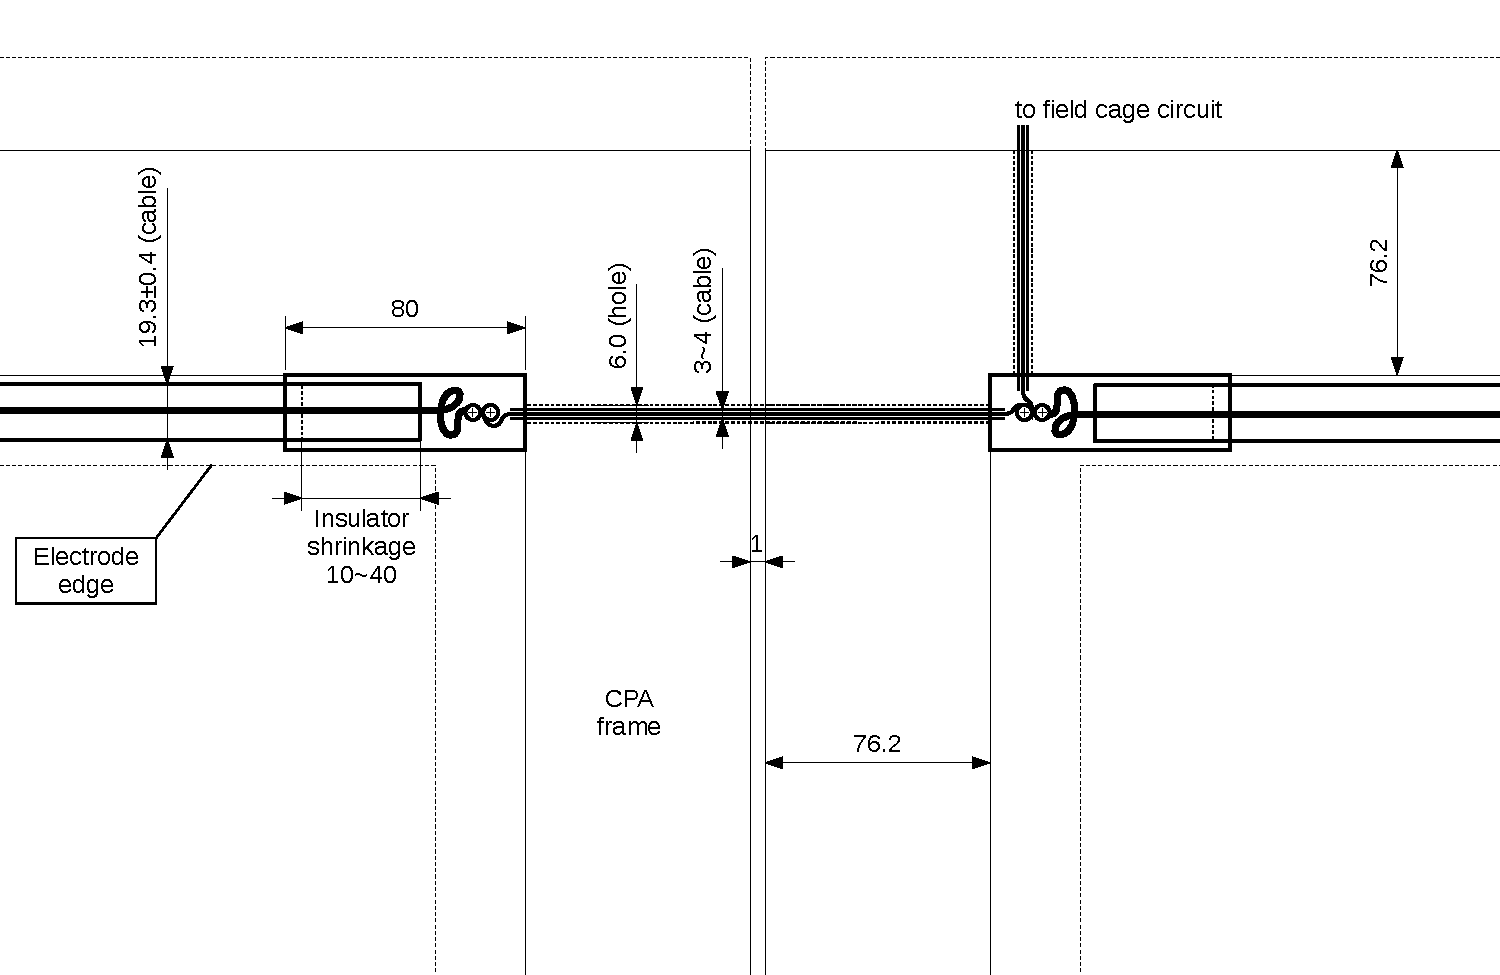
\includegraphics[height=0.3\textheight]{HVbus-connections}
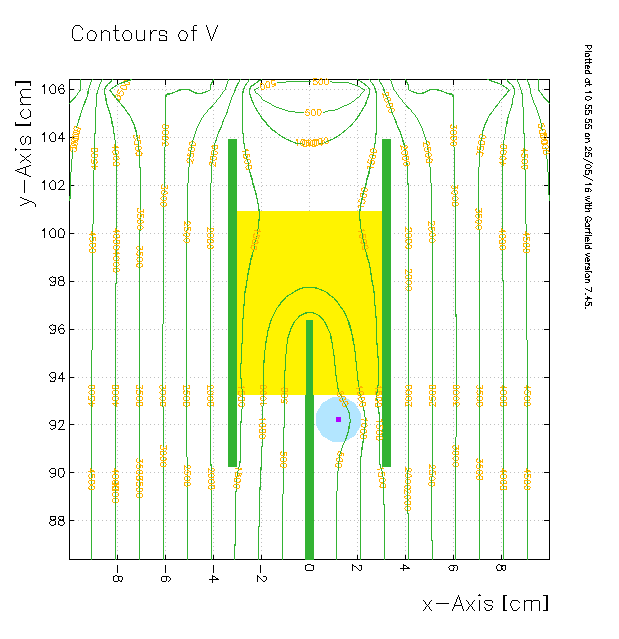
\includegraphics[height=0.3\textheight]{HVbus-vcontour}
\end{cdrfigure}

\subsection{HV monitoring}

HV circuit monitoring devices include a toroid transformer to detect
spikes and noise in the current draw and a monitoring point at the end
of the field cage resistor chain, which also provides a means to
control field shaping around the edge of the
APA.

\subsection{HV testing}

To ensure safe and reliable operation, the HV components will be
tested at a much higher voltage than expected in routine operation
($\sim\SI{250}{kV}$) in LAr. Among these tests will be a planned
``full scale'' high voltage test at Fermilab in which all components
are subjected to the full voltage and field in liquid argon in the
35-ton cryostat.


